\documentclass{article}
\usepackage[utf8]{inputenc}
\usepackage{amsthm}
\usepackage{hyperref}
\usepackage{pdfpages}
\begin{document}

\begin{titlepage}
    \begin{center}
        \vspace*{1cm}
            
        \Huge
        \textbf{Lab 9 Report}
            
        \vspace{0.5cm}
        \LARGE
        Analysis of the Chemical Composition of Various Cannabis Products
            
        \vspace{1.5cm}
            
        \textbf{Wenqi Guo*}, Austin and Mathew
        \begin{small}
            \url{https://scholar.google.com/citations?user=4YWcPZoAAAAJ}
        \end{small}

            
        \vfill
            
TA name:
Adebowale, Adeyemi

            
        \vspace{0.8cm}
            

            
        \Large
        Department of Chemistry\\
        University of British Columbia\\
        Dec 13, 2022
            
    \end{center}
\end{titlepage}
Code and raw \LaTeX \; of this lab report can be found on \url{https://github.com/weathon/Chem-Lab-9}
\section*{Abstract}

Cannabis markets are increasing \cite{Lab Manuel} in both Canada and the US.   In this paper, we analyzed the data set from the publication  \cite{dataset1} and \cite{dataset2} using various methods. This dataset contains the composition of 12 cannabis strains using HPLC-UV. \cite{Lab Manuel, dataset1, dataset2} We first did an ANOVA of different substances in different strains. 
We then used metaboanalyst.ca to do the Pearson Correlation on the dataset. Then we used Python to analyze the dataset using PCA and SAM. We find that ~~~~

\\ \textbf{Keywords: } Cannabis, Statistical Analysis, Dataset, Significance Analysis of Microarrays, Principal Component Analysis
\newpage
\section{Introduction}
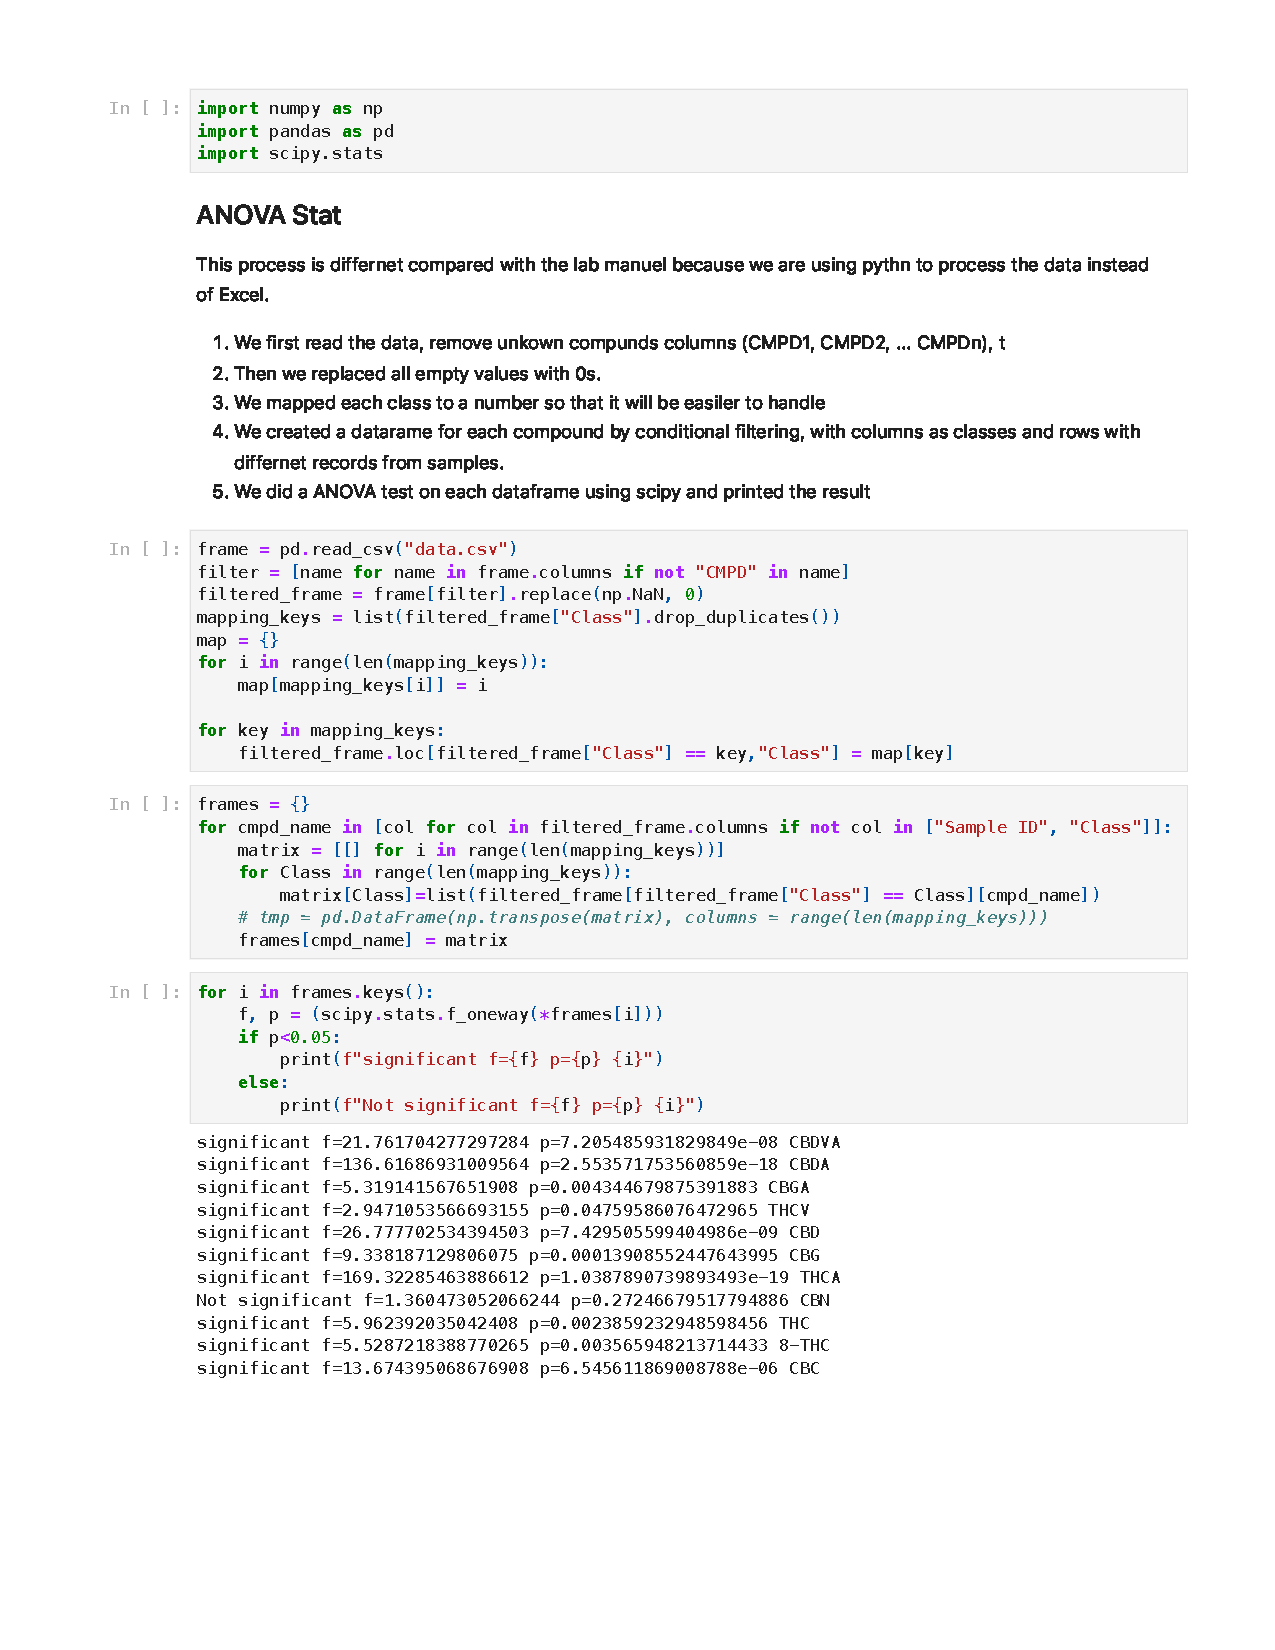
\includepdf[scale=0.8, offset=0 -2cm, pagecommand=\section{Materials and Methods} These process are based on \cite{Lab Manuel}. We converted the Excel file into a CSV file.]{main.pdf}
\subsection*{AetaboanAlyst}
We used MetaboanAlyst for the rest of the data analytics.  We used the same dataset as we did in the last section. 


\begin{enumerate}
    \item We uploaded the CSV file to AetaboanAlyst with one var statistical analytics with the data type of concentration and sample of "rows (unpaired)." 
    \item We then skipped the missing value filling.
    \item We then normalized the data with "auto-scaling"
    \item In the statistical analysis model, 
\end{enumerate}


\section{Result}
\section{Discussion}
\begin{thebibliography}{9}
\bibitem{Lab Manuel}


\bibitem{dataset1}
Mudge, E.M.; Brown, P.N.; Murch, S.J. The Terroir of Cannabis: Terpene Metabolomics as a Tool
 to Understand Cannabis Selections. Planta Medica. 2019. DOI: 10.1055/a-0915-2550

\bibitem{dataset2}

Mudge, E.M.; Murch, S.J.; Brown, P.N. Chemometric analysis of cannabinoids: chemotaxonomy
 and domestication syndrome. Scientific Reports. 2018. 8, 13090. DOI:10.1038/s41598
 018-31120-2 1. 
\end{thebibliography}

\end{document}
